\chapter{Вероятность, информация и энтропия}

\lectureoverview{Статистическая механика начинается там, где микроскопический закон встречается с неполным знанием. Сначала мы придадим вероятности точный смысл, затем спросим, как само детерминированное движение задаёт вероятности, как законы сохранения разбивают пространство состояний и почему динамика, сохраняющая информацию, естественным образом приводит к энтропии. Первый и нулевой законы вступают в игру лишь после того, как эта структура установлена.}

\section{Зачем нужна статистическая механика?}

Статистическую механику иногда описывают как старую физику. Такое описание упускает главное. Она и досовременна, и современна и, вероятно, останется полезной в любой постсовременной физике, которая придёт на смену известным нам теориям. Частные модели возникают и исчезают; второй закон термодинамики снова и снова сохранялся как ориентир. Всякий раз, когда предлагаемое описание природы как будто создаёт порядок даром, принципиально уничтожает информацию или сводит замкнутую систему к неестественно простому состоянию, второй закон предупреждает нас, что что-то было упущено.

Эта дисциплина может казаться менее эффектной, чем вновь открытая частица, но она по меньшей мере столь же глубока и гораздо более обща. Газы, жидкости, твёрдые тела, излучение, чёрные дыры, информация и квантовые поля — всё это требует статистических рассуждений. Более того, без неё нельзя было бы понять экспериментальный аппарат, использованный для открытия частиц. Вот почему поколения сильных физиков овладевали статистической механикой, даже когда их основная работа лежала в других областях: эта дисциплина полезна, но, кроме того, необычайно красива.

Чтобы понять, зачем она нужна, начнём с идеала, задаваемого механикой. Замкнутая система — это либо вся рассматриваемая вселенная, либо подсистема, достаточно хорошо изолированная, чтобы окружение на неё не влияло. Если нам известны её начальное состояние и закон эволюции, то классическая механика даёт полное предсказание. Квантовая механика изменяет то, что может быть предсказано, но и в ней есть точно определённое состояние и закон, предсказывающий максимум информации, допускаемый теорией.

Между предсказанием в принципе и полезным пониманием существует резкое различие. Список положений и скоростей всех молекул в этой комнате был бы невероятно длинным, почти сразу изменился бы и ответил бы лишь на немногие из вопросов, которые нас действительно интересуют. Поэтому точные микроскопические законы могут одновременно обладать полной предсказательной силой и быть практически бесполезными.

Статистическая механика — это теория вероятностей, применённая к данной физической ситуации. Она становится необходимой, когда начальное состояние известно не с совершенной точностью, когда закон известен лишь приближённо, когда система открыта или просто когда число микроскопических переменных слишком велико, чтобы их отслеживать. Ничто из этого не означает слабости предсказаний. Большие числа часто делают статистические предсказания чрезвычайно точными.

Рассмотрим изолированный ящик с газом. Мы не можем предсказать траекторию каждой молекулы, однако немногие макроскопические данные позволяют нам с высокой точностью предсказывать давление, энергию и многие другие макроскопические величины. Неопределёнными остаются флуктуации. В непредсказуемый момент малая область может содержать больше молекул, чем в среднем, тогда как другая содержит меньше. Такое событие лежит в хвосте распределения вероятностей: оно маловероятно, но не запрещено. Мы можем вычислить, как часто должны происходить такие флуктуации, не предсказывая момент конкретного появления одной из них.

Подбрасывание монеты демонстрирует то же различие. В миллиарде честных бросков числа орлов и решек будут близки друг к другу. Длинная серия орлов в конце концов возникнет, если бросать достаточно долго, но теория вероятностей предсказывает её частоту, а не указывает заранее, когда именно это произойдёт. Статистическая механика предназначена для систем, элементы которых слишком малы, слишком многочисленны или и то и другое одновременно.

В этом курсе будут развиты законы, а также их приложения к веществу. Эта дисциплина вознаграждает многократное изучение: её изучают, забывают часть материала, а затем изучают снова, уже глубже понимая, какие идеи являются фундаментальными. Мы начнём с идеи, которая определяет всё дальнейшее.

\section{Вероятность как исходный язык}

Почему вероятность работает, не объясняется самим исчислением вероятностей. Вероятностное предсказание может не оправдаться в отдельном испытании; именно это и означает, что исход возможен, но маловероятен. Теория говорит нам, как распределены исключения. Она не устраняет их. Поэтому мы принимаем вероятность как исходное понятие и формулируем правила, которым она подчиняется.

\subsection{Состояния и нормировка}

Пусть \(i\) обозначает возможный исход или возможное состояние системы. Для одной монеты \(i\) может означать орёл или решку. Для одного игрального кубика этот индекс может принимать значения от \(1\) до \(6\). Для двух кубиков пара индексов задаёт оба выпавших значения. Мы начнём с конечного дискретного пространства состояний,
\begin{equation}
 i=1,\ldots,N,
\end{equation}
а позже перейдём к бесконечному числу состояний и к непрерывному множеству состояний.

Незнание не означает, что у системы нет состояния. Оно означает, что мы не знаем, какое именно состояние она имеет, поэтому каждой возможности мы приписываем вероятность \(p_i\). Основные правила таковы:
\begin{align}
 p_i &\geq 0, \label{eq:sm1-prob-positive}\\
 \sum_{i=1}^{N}p_i &=1. \label{eq:sm1-prob-normalization}
\end{align}
Альтернативы взаимно исключают друг друга и исчерпывают все возможности: реализуется ровно одна из них. Отрицательным вероятностям здесь места нет, а сумма равна единице, потому что должен реализоваться некоторый допустимый исход.

\subsection{Частота и закон больших чисел}

Вероятность связывается с экспериментом посредством повторных испытаний. Предположим, что один и тот же эксперимент проводится \(N_{\mathrm{trials}}\) раз, и пусть \(N(i)\) — число испытаний, в которых получается исход \(i\). Тогда частотная интерпретация имеет вид
\begin{equation}
 p_i=
 \lim_{N_{\mathrm{trials}}\to\infty}
 \frac{N(i)}{N_{\mathrm{trials}}}.
 \label{eq:sm1-frequency}
\end{equation}
Это физическая гипотеза, выраженная через идеальный предел. Ни одна лаборатория не проводит бесконечно много экспериментов. Утверждение состоит в том, что при достаточно большом числе испытаний отношение становится достаточно близким к \(p_i\) для нужного предсказания. Конечные выборки флуктуируют вокруг предельного значения.

\subsection{Средние значения}

Теперь сопоставим каждому состоянию число \(f(i)\). Это может быть энергия, импульс или любая другая величина, которую мы хотим измерить. Математическое ожидание этой величины равно
\begin{equation}
 \langle f\rangle=\sum_i f(i)p_i.
 \label{eq:sm1-expectation}
\end{equation}
Обозначение угловыми скобками удобно и вне квантовой механики. На языке частот то же среднее имеет вид
\begin{equation}
 \langle f\rangle
 =
 \lim_{N_{\mathrm{trials}}\to\infty}
 \frac{1}{N_{\mathrm{trials}}}
 \sum_i f(i)N(i).
 \label{eq:sm1-frequency-average}
\end{equation}

Для монеты определим
\begin{equation}
 f(\mathrm{H})=+1,
 \qquad
 f(\mathrm{T})=-1.
\end{equation}
Если орёл и решка имеют вероятности \(1/2\) каждая, то
\begin{equation}
 \langle f\rangle
 =(+1)\frac12+(-1)\frac12=0.
\end{equation}
Среднее не обязано быть возможным исходом. Монета никогда не падает на нуль; нуль характеризует распределение её двух возможных значений.

Этот краткий экскурс фиксирует словарь, используемый во всей дисциплине: состояния, вероятности, частоты и средние значения.

\section{Три способа задания вероятностей}

\subsection{Симметрия}

Почему мы обычно приписываем двум сторонам монеты равные вероятности? Первый ответ — симметрия. Переворачивание почти идеальной монеты меняет местами орёл и решку, не изменяя самого эксперимента. Тогда нет физических оснований предпочесть какой-либо из этих исходов. Реальная метка или несовершенство вносит крошечное смещение, но симметричная модель передаёт суть задуманного эксперимента:
\begin{equation}
 p(\mathrm{H})=p(\mathrm{T})=\frac12.
\end{equation}

Тот же аргумент даёт вероятность \(1/6\) для каждой грани симметричного кубика. В более общем случае конфигурациям, связанным симметрией, приписывают равные вероятности, если только некоторая дополнительная информация не нарушает эту симметрию.

\subsection{Эксперимент}

Кубик неправильной формы не имеет симметрии, переставляющей все шесть граней. В этом случае одна лишь симметрия ответа не даёт. Можно располагать более глубокой механической моделью, которая предсказывает смещение, но в отсутствие такой модели добросовестная процедура является экспериментальной: много раз бросать кубик, записывать частоты, ждать, пока они стабилизируются, и использовать полученную таблицу вероятностей в последующих предсказаниях.

Симметрия и эксперимент — не конкурирующие определения. Это два источника информации о распределении вероятностей. Статистическая механика будет в значительной степени опираться на симметрию, но динамика даёт и третий путь.

\subsection{Вероятность из детерминированного движения}

Представьте себе объект неправильной формы с шестью цветными конфигурациями. Через фиксированные дискретные интервалы времени его состояние изменяется согласно определённому закону переходов:
\begin{equation}
 R\longrightarrow B\longrightarrow Y\longrightarrow G
 \longrightarrow O\longrightarrow P\longrightarrow R.
 \label{eq:sm1-six-cycle}
\end{equation}
Сам объект не обязан обладать какой-либо геометрической симметрией. Закон лишь указывает, какая конфигурация следует за данной конфигурацией.

\begin{figure}[htbp]
\centering
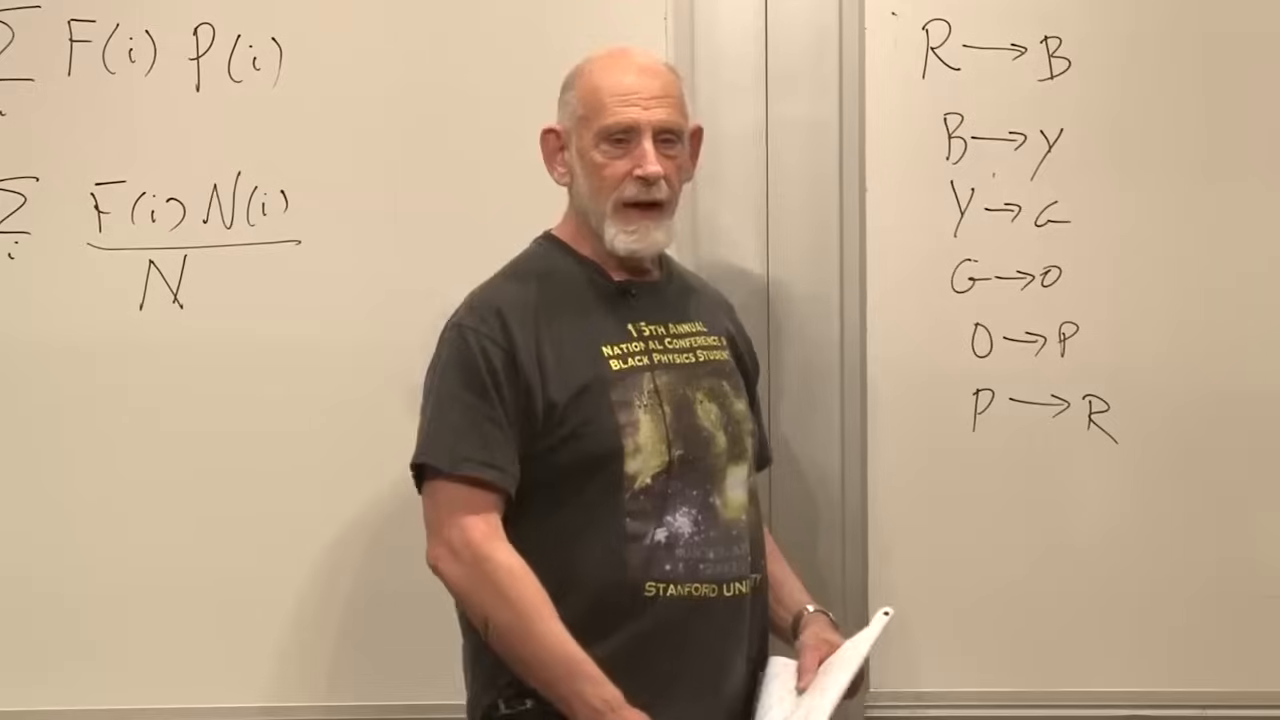
\includegraphics[width=0.92\textwidth]{lecture_01_figure_02.png}
\caption{Формулы для средних значений остаются на левой доске, а шесть детерминированных цветовых переходов перечислены на правой.}
\lectureframe{00:26:28}
\end{figure}

Список на доске становится нагляднее, если изобразить его как ориентированный цикл:
\begin{figure}[htbp]
\centering
\begin{tikzpicture}[
  >=Latex,
  state/.style={draw,circle,minimum size=8mm,inner sep=1pt}
]
\node[state] (R) at (90:2.2) {$R$};
\node[state] (B) at (30:2.2) {$B$};
\node[state] (Y) at (-30:2.2) {$Y$};
\node[state] (G) at (-90:2.2) {$G$};
\node[state] (O) at (-150:2.2) {$O$};
\node[state] (P) at (150:2.2) {$P$};
\draw[->] (R) -- (B);
\draw[->] (B) -- (Y);
\draw[->] (Y) -- (G);
\draw[->] (G) -- (O);
\draw[->] (O) -- (P);
\draw[->] (P) -- (R);
\end{tikzpicture}
\caption{Одна орбита из шести состояний. В течение каждого периода каждое состояние посещается один раз.}
\label{fig:sm1-six-cycle}
\end{figure}

Предположим, что начальное состояние нам неизвестно и что мы делаем моментальный снимок в неизвестный момент времени. Поскольку каждый шаг длится одинаково долго, система проводит одну шестую периода в каждом цвете:
\begin{equation}
 p(R)=p(B)=p(Y)=p(G)=p(O)=p(P)=\frac16.
 \label{eq:sm1-uniform-cycle}
\end{equation}
Это равенство следует не из формы объекта. Оно следует из равного времени, проводимого в состояниях.

Мы можем переставить стрелки и получить другой микроскопический закон, при этом по-прежнему образуя один цикл из шести состояний. Подробная последовательность меняется, но вероятность, получаемая по снимку, остается \(1/6\), потому что каждое состояние по-прежнему встречается один раз за период. Следовательно, для этого предсказания не нужны ни начальная точка, ни детальный порядок. Достаточно лишь структуры орбиты и равного времени каждого обновления.

\begin{classroomqa}
\classquestion{Если объект несимметричен, в каком смысле правомерно приписывать каждому цвету вероятность \(1/6\)?}
\lecturerresponse{Это приписывание является динамическим, а не геометрическим. Снимок, сделанный при неизвестной фазе шестишаговой орбиты, выбирает один из шести равных по времени интервалов. Существенная эквивалентность здесь — между положениями на орбите, а не между гранями объекта. Если бы времена пребывания были неодинаковы, то и вероятности были бы неодинаковыми.
\lecturetimestamp{00:27:11--00:29:49}}
\end{classroomqa}

\section{Несвязные циклы и сохраняющиеся величины}

Детерминистический закон не обязан помещать все состояния на одну орбиту. Рассмотрим два несвязанных цикла,
\begin{equation}
 R\longrightarrow B\longrightarrow G\longrightarrow R,
 \qquad
 P\longrightarrow Y\longrightarrow O\longrightarrow P.
 \label{eq:sm1-two-cycles}
\end{equation}
Если мы знаем, что система находится на первом цикле, то
\begin{equation}
 \begin{aligned}
 p(R)=p(B)=p(G)&=\frac13,\\
 p(P)=p(Y)=p(O)&=0.
 \end{aligned}
\end{equation}
Знание того, что она находится на втором цикле, дает обратное присвоение вероятностей.

В более общем случае требуются априорные веса. Обозначим циклы \(+1\) и \(-1\), а их вероятности — \(p_+\) и \(p_-\), причем
\begin{equation}
 p_++p_-=1.
\end{equation}
Тогда
\begin{align}
 p(R)=p(B)=p(G)&=\frac{p_+}{3},\\
 p(P)=p(Y)=p(O)&=\frac{p_-}{3}.
 \label{eq:sm1-sector-weights}
\end{align}
Множители \(1/3\) следуют из движения внутри цикла. Числа \(p_+\) и \(p_-\) — нет. Они должны следовать из дополнительного знания, возможно из другого эксперимента или из другой системы, которая выбирает начальный сектор.

Метки \(+1\) и \(-1\) задают сохраняющуюся величину: если система стартовала на одном цикле, закон обновления никогда не переводит ее на другой. Эту величину можно назвать энергией или дать ей условное имя, например \emph{зильч}. Ее название второстепенно. Сохранение означает, что пространство состояний разбивается на области, которые динамика не может пересечь.

Циклы не обязаны содержать одинаковое число состояний. Орбита из четырех состояний и орбита из двух состояний все равно задают два инвариантных сектора. Тогда выборка по равным временам дает \(1/4\) внутри первого и \(1/2\) внутри второго, причем в каждом случае это умножается на априорную вероятность соответствующего сектора. Статистическая механика должна ответить на два логически различных вопроса:
\begin{enumerate}
\item Если дан инвариантный сектор, сколько времени динамика проводит в его состояниях?
\item Какую вероятность следует приписать самому инвариантному сектору?
\end{enumerate}

\begin{classroomqa}
\audiencequestion{Предполагаем ли мы, что всем состояниям внутри одного инвариантного сектора приписывается одна и та же вероятность?}
\lecturerresponse{Для приведенных здесь дискретных модельных законов — да, потому что каждое состояние длится один и тот же интервал времени, а движение детерминистично. Неизвестной остается начальная фаза орбиты. Детектор с миллисекундным разрешением по времени не может различить микросекундные обновления, хотя достаточно быстрый снимок все же может определить, какое состояние было зафиксировано. В более общей системе неодинаковые времена пребывания нужно учитывать явно.
\lecturetimestamp{00:36:16--00:37:17}}
\end{classroomqa}

\begin{classroomqa}
\audiencequestion{Если сделаны два снимка и первый идентифицирует один цикл, должен ли второй идентифицировать тот же цикл?}
\lecturerresponse{Да. Именно это и означает сохранение. Как только измерение определяет значение сохраняющейся величины, будущие вероятности можно условить на это значение, а состояния в другом секторе получают нулевую вероятность.
\lecturetimestamp{00:37:18--00:37:45}}
\end{classroomqa}

\subsection{Энергия, распределенная между двумя системами}

Теперь заменим абстрактную метку энергией. Один изолированный ящик — это замкнутая система, и его энергия сохраняется. Два изолированных ящика имеют две независимо сохраняющиеся энергии, поскольку они не взаимодействуют. Если соединить их узким проходом, допускающим перетекание энергии, отдельные энергии могут изменяться, тогда как полная остается фиксированной.

\begin{figure}[htbp]
\centering
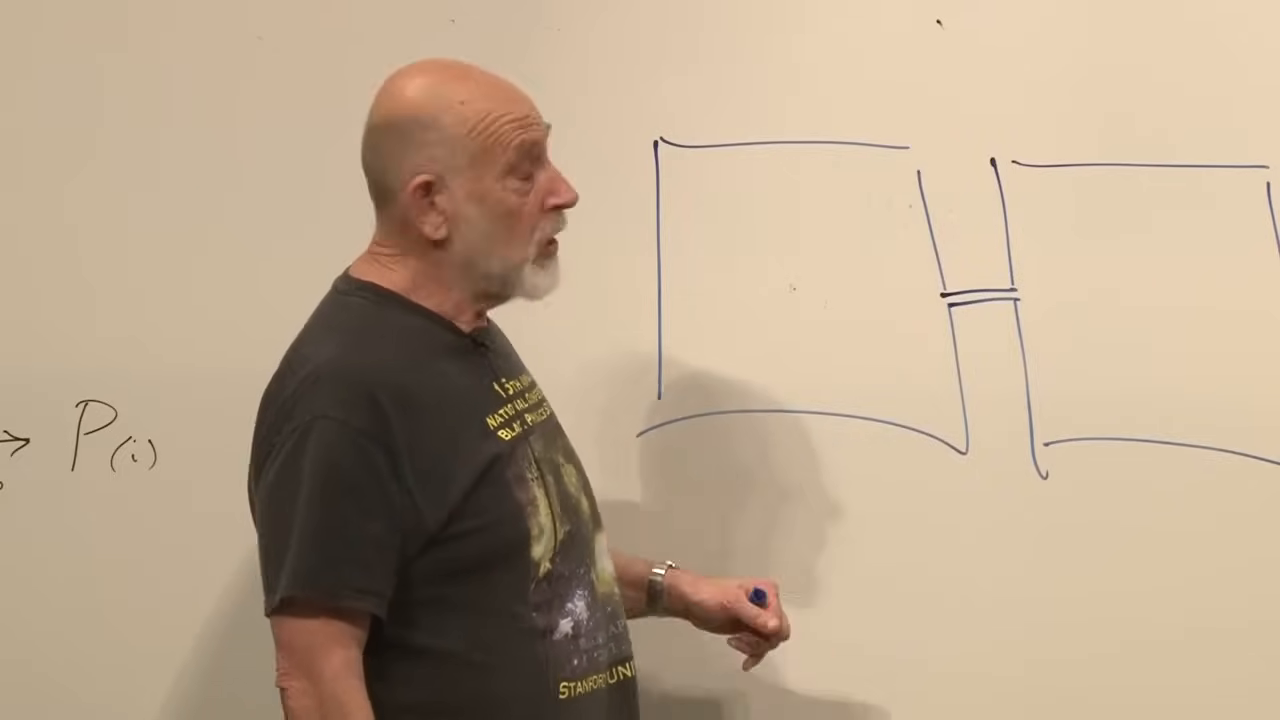
\includegraphics[width=0.92\textwidth]{lecture_01_figure_03.png}
\caption{Две подсистемы, соединенные узким каналом, через который может проходить энергия.}
\lectureframe{00:39:19}
\end{figure}

\begin{figure}[htbp]
\centering
\begin{tikzpicture}[>=Latex]
\draw[thick,rounded corners=4pt] (-4,1.8) rectangle (-0.7,-1.5);
\draw[thick,rounded corners=4pt] (0.7,1.5) rectangle (4,-1.8);
\draw[thick] (-0.7,0.45) -- (0.7,0.45);
\draw[thick] (-0.7,-0.35) -- (0.7,-0.35);
\draw[<->,very thick] (-0.45,0.05) -- (0.45,0.05);
\node at (-2.35,0.15) {subsystem \(1\)};
\node at (2.35,-0.15) {subsystem \(2\)};
\node[above] at (0,0.5) {energy exchange};
\end{tikzpicture}
\caption{После открытия соединения сохраняется только \(E_1+E_2\). Распределение энергии становится вероятностной задачей.}
\label{fig:sm1-connected-systems}
\end{figure}

При заданной полной энергии можно спросить, какова вероятность того, что подсистема \(1\) имеет \(E_1\), тогда как подсистема \(2\) имеет остаток. У одинаковых ящиков средние энергии должны быть одинаковы, но среднее не исчерпывает всего распределения. Поэтому один из способов определить вероятности для подсистемы состоит в том, чтобы вложить ее в более крупную замкнутую систему, закон сохранения которой дает недостающую информацию. Эта конструкция будет снова и снова появляться в статистической механике.

\section{Хорошие законы, плохие законы и минус первый закон}

Не всякое детерминистическое правило обновления допустимо в качестве фундаментального закона. Рассмотрим отображение
\begin{equation}
 \begin{aligned}
 R&\mapsto R,& B&\mapsto R,& Y&\mapsto R,\\
 G&\mapsto R,& O&\mapsto R,& P&\mapsto R.
 \end{aligned}
 \label{eq:sm1-all-to-red}
\end{equation}
Оно безупречно предсказывает будущее: через один шаг состояние будет красным. В обратном направлении оно не работает. Когда система находится в красном состоянии, ничто не позволяет узнать, пришла ли она из синего, желтого, зеленого, оранжевого, фиолетового или из самого красного.

\begin{figure}[htbp]
\centering
\begin{tikzpicture}[
  >=Latex,
  state/.style={draw,circle,minimum size=8mm,inner sep=1pt}
]
\node[state,fill=red!12] (R) at (0,0) {$R$};
\node[state] (B) at (-3,1.6) {$B$};
\node[state] (Y) at (-3,0) {$Y$};
\node[state] (G) at (-3,-1.6) {$G$};
\node[state] (O) at (3,1.6) {$O$};
\node[state] (P) at (3,-1.6) {$P$};
\draw[->] (B) -- (R);
\draw[->] (Y) -- (R);
\draw[->] (G) -- (R);
\draw[->] (O) -- (R);
\draw[->] (P) -- (R);
\draw[->,loop above] (R) to (R);
\end{tikzpicture}
\caption{Закон типа многие-к-одному предсказывает следующее состояние, но стирает различия между возможными прошлыми состояниями.}
\label{fig:sm1-bad-law}
\end{figure}

Напротив, замкнутый цикл сохраняет запись. Если известно прошедшее время, мы можем проследить эволюцию состояния вперед или назад, даже по прошествии многих тысяч периодов. Закон сохраняет различия между начальными условиями. Сасскинд называет это требование \emph{минус первым законом физики}: информация фундаментально не теряется.

Для конечного дискретного пространства состояний критерий по диаграмме прост:
\begin{quote}
У каждого состояния хорошего закона есть ровно одна исходящая и ровно одна входящая стрелка.
\end{quote}
Исходящая стрелка определяет будущее; входящая восстанавливает прошлое. Математически обновление — это перестановка состояний.

\subsection{Трение — лишь кажущийся контрпример}

Непрерывным аналогом служит теорема Лиувилля. Трение, по-видимому, ей противоречит. Пустите ластик скользить по столу, и, где бы он ни находился вначале, в конце концов он остановится. Схематическое уравнение сопротивления имеет вид
\begin{equation}
 m\ddot x=-\gamma\dot x,
 \qquad \gamma>0.
 \label{eq:sm1-drag}
\end{equation}
Его скорость экспоненциально убывает. Если бы это был самый фундаментальный закон для каждой частицы в герметически закрытой комнате, всякое движение затухало бы, температура падала бы до нуля, а многие начальные состояния схлопывались бы в одно конечное состояние. Закон сохранения энергии нарушался бы, информация исчезала бы, а беспорядок уменьшался бы. Это была бы непрерывная версия того, что всё приходит в красное состояние.

Реальное трение так не действует. Ластик нагревает стол, самого себя и окружающую среду. Микроскопические координаты и импульсы сохраняют различия, утраченные в видимом движении. Трение — это эффективное уравнение для подсистемы после того, как ненаблюдаемые степени свободы были отброшены; это не фундаментальный диссипативный закон для полной замкнутой системы.

\begin{classroomqa}
\classquestion{Что представляет собой дифференциальное уравнение
\(m\ddot x=-\gamma\dot x\) и почему оно не является фундаментальным законом
замкнутой системы?}
\lecturerresponse{Оно описывает вязкое сопротивление. Само по себе оно заставляет всякую скорость стремиться к нулю, что заставило бы газ остыть до нуля независимо от его начальной температуры. В реальном замкнутом описании потерянные механическая энергия и информация переходят в микроскопические степени свободы. Уравнение сопротивления надежно только после того, как эти переменные исключены из описания.
\lecturetimestamp{00:44:40--00:48:56}}
\end{classroomqa}

\section{Занятые состояния и первая энтропия}

Сохранению информации соответствует эквивалентное вероятностное утверждение. Предположим, что \(M\) из \(N\) состояний имеют одинаковую вероятность,
\begin{equation}
 p_i=
 \begin{cases}
 1/M, & i\text{ in the occupied set},\\
 0, & i\text{ outside it}.
 \end{cases}
 \label{eq:sm1-uniform-occupied}
\end{equation}
Обновление, сохраняющее информацию, может переставить, какие именно состояния заняты, но не может слить их воедино. В любой более поздний момент по-прежнему имеется \(M\) состояний с вероятностью \(1/M\). Плохое отображение \eqref{eq:sm1-all-to-red}, напротив, может схлопнуть многие занятые состояния в одно.

Число \(M\) служит мерой незнания. Если \(M=N\), возможно каждое состояние и наше незнание максимально. Если \(M=1\), микроскопическое состояние известно точно. Поэтому первое определение энтропии таково
\begin{equation}
 S=\log M.
 \label{eq:sm1-entropy-logm}
\end{equation}
Отсюда
\begin{equation}
 S_{\max}=\log N,
 \qquad
 S_{\min}=0.
\end{equation}
Если пространство состояний бесконечно, конечной верхней границы может и не быть.

В этом изложении энтропия появляется раньше температуры и даже раньше формулировки закона сохранения энергии. В этом смысле она более первична. Однако она не является свойством одной лишь механической системы. Она совместно зависит от системы и от распределения вероятностей, представляющего то, что известно. Одной и той же механической системе наблюдатели, располагающие разной информацией, могут приписывать разные энтропии.

При точной микроскопической эволюции занятые состояния лишь переставляются, поэтому эта мелкозернистая энтропия сохраняется. На практике мы теряем информацию о времени, отбрасываем корреляции и не можем отслеживать огромное число переменных. Тогда наше распределение вероятности размазывается по большему числу альтернатив, и энтропия, приписываемая грубому описанию, возрастает. Чтобы пригодное нам описание теряло информацию, вовсе не требуется, чтобы уравнения её уничтожали.

\begin{classroomqa}
\classquestion{Какова максимально возможная энтропия конечной системы с \(N\) состояниями?}
\lecturerresponse{Она равна \(\log N\) и достигается, когда все \(N\) состояний равновероятны. Наименьшая энтропия равна нулю; она достигается, когда вероятность одного состояния равна единице. Следовательно, энтропия характеризует как состояние знания, так и доступное пространство состояний.
\lecturetimestamp{00:56:46--00:58:19}}
\end{classroomqa}

\section{Поток Лиувилля в непрерывном фазовом пространстве}

Для частиц с непрерывными координатами и импульсами микроскопическое состояние есть точка в фазовом пространстве. Координаты мы обозначаем как \(q_a\), а сопряжённые им импульсы — как \(p_a\). Для многих частиц осей оказывается чрезвычайно много; двумерный рисунок, где есть лишь одна \(q\) и один \(p\), служит только условной иллюстрацией. Размерность фазового пространства чётна, потому что каждой координате соответствует сопряжённый импульс.

Предположим, что наше знание представлено областью \(\Omega_0\): плотность вероятности внутри этой области постоянна, а вне её равна нулю. Например, знание того, что каждая частица находится в комнате, ограничивает координаты положения, тогда как ограничения на их скорости ограничивают импульсные координаты.

Гамильтонова эволюция переносит каждую точку фазового пространства вдоль траектории. Близкие точки переходят в близкие точки, и занятая область течёт как порция несжимаемой жидкости:
\begin{figure}[htbp]
\centering
\begin{tikzpicture}[>=Latex,scale=0.95]
\draw[->] (-4.2,0) -- (4.3,0) node[right] {$q$};
\draw[->] (-3.7,-2.2) -- (-3.7,2.4) node[above] {$p$};
\draw[fill=blue!12,thick]
  (-3.0,-0.5) .. controls (-2.7,1.0) and (-1.3,1.2) .. (-0.9,0.1)
  .. controls (-0.6,-1.0) and (-2.2,-1.4) .. cycle;
\node at (-1.9,0.0) {$\Omega_0$};
\draw[->,very thick] (-0.3,0.2) -- (0.8,0.2);
\draw[fill=orange!15,thick]
  (1.2,-1.1) .. controls (1.5,0.3) and (2.3,1.8) .. (3.2,1.1)
  .. controls (3.6,0.7) and (2.8,-0.4) .. (2.5,-1.5)
  .. controls (2.1,-1.8) and (1.5,-1.6) .. cycle;
\node at (2.35,0.1) {$\Omega_t$};
\end{tikzpicture}
\caption{Гамильтонов поток может растягивать и сдвигать занятую область фазового пространства, но сохраняет её объём.}
\label{fig:sm1-liouville-flow}
\end{figure}

Теорема Лиувилля утверждает:
\begin{equation}
 \operatorname{Vol}(\Omega_t)
 =
 \operatorname{Vol}(\Omega_0).
 \label{eq:sm1-liouville-volume}
\end{equation}
Если начальная плотность равномерна на \(\Omega_0\), то перенесённая плотность равномерна на \(\Omega_t\). Это непрерывный аналог сохранения числа и весов занятых дискретных состояний.

Эта теорема также геометрически разрешает загадку трения. Если смотреть только на наблюдаемый импульс ластика, облако возможностей как будто сжимается к \(p=0\). В полном фазовом пространстве это облако распространяется по координатам и импульсам молекул в ластике и столе. Проекция может сжиматься, тогда как полный многомерный объём остаётся постоянным.

\begin{classroomqa}
\classquestion{Если каждая наблюдаемая траектория стремится к покою, схлопнулась ли занятая область фазового пространства на ось \(p=0\)?}
\lecturerresponse{Только в редуцированной проекции. Полная система включает микроскопические переменные стола, ластика и окружающей среды. По мере того как диапазон видимого импульса сужается, распределение растекается по этим скрытым направлениям. Теорема Лиувилля относится к полному замкнутому фазовому пространству, а не к неполному набору макроскопических переменных.
\lecturetimestamp{01:04:37--01:06:29}}
\end{classroomqa}

\section{От минус первого закона к первому закону}

\subsection{Кратко о нулевом законе}

Прежде чем формулировать первый закон, полезно назвать нулевой. Тепловое равновесие ещё не определено, поэтому пока этот закон является лишь структурным утверждением:
\begin{quote}
Если система \(A\) находится в тепловом равновесии с \(B\), а \(B\) находится в тепловом равновесии с \(C\), то \(A\) находится в тепловом равновесии с \(C\).
\end{quote}
Эта транзитивность позже сделает возможным введение температуры. Пока же мы оставим её в стороне.

\subsection{Сохранение энергии}

Первый закон для замкнутой системы просто гласит:
\begin{equation}
 \frac{dE}{dt}=0.
 \label{eq:sm1-first-law}
\end{equation}
Его компактная форма скрывает его силу. Энергия является сохраняющейся величиной, и слово энергия позже приобретёт более содержательный термодинамический смысл.

Если замкнутая система состоит из двух частей и их энергии аддитивны,
\begin{equation}
 E=E_1+E_2,
\end{equation}
то
\begin{equation}
 \frac{dE_1}{dt}+\frac{dE_2}{dt}=0,
 \qquad\text{or}\qquad
 \frac{dE_1}{dt}=-\frac{dE_2}{dt}.
 \label{eq:sm1-energy-exchange}
\end{equation}
Вторая форма делает обмен явным: энергия, потерянная одной подсистемой, приобретается другой.

Предположение об аддитивности требует осторожности. У двух гравитационно взаимодействующих частиц есть индивидуальные кинетические энергии, но их взаимодействие даёт потенциальную энергию, принадлежащую паре. Полная энергия сохраняется, хотя её нельзя точно записать как энергию одного тела плюс энергию другого.

Термодинамика часто допускает превосходное аддитивное приближение, потому что объёмная энергия масштабируется с объёмом, тогда как энергия короткодействующего взаимодействия между большими соседними частями масштабируется главным образом с площадью их соприкосновения. Разделите большой стол на блоки: внутренняя энергия каждого блока — объёмный эффект, а взаимодействие между соседними блоками — поверхностный эффект. Для больших блоков этот вклад сравнительно мал. Уравнение
\eqref{eq:sm1-first-law} точно для замкнутого целого; форма для подсистем
\eqref{eq:sm1-energy-exchange} предполагает пренебрежимо малую энергию взаимодействия.

\begin{classroomqa}
\audiencequestion{Нормировка \(\sum_i p_i=1\) также предполагает, что перечисленные исходы взаимно исключают друг друга?}
\lecturerresponse{Да. Метка состояния определяется так, чтобы альтернативы не перекрывались: если игральная кость находится в жёлтом состоянии, то она не находится одновременно в красном состоянии. В обычном языке цвета могут смешиваться, но разбиение на состояния, используемое при вычислении вероятности, должно состоять из взаимно исключающих альтернатив.
\lecturetimestamp{01:12:14--01:12:55}}
\end{classroomqa}

\section{Возвращение к энтропии}

Теперь лекция явно возвращается к тому, что осталось незавершённым. Температура, хотя и знакома нашим чувствам, является производной величиной. Прежде чем можно будет чётко определить температуру, должны быть введены энтропия и энергия.

\subsection{Общие распределения вероятности}

Специальное определение \(S=\log M\) применимо, когда \(M\) состояний равновероятны, а все остальные имеют нулевую вероятность. Общее распределение не обязано иметь прямоугольную форму. Его веса могут изменяться по меткам состояний плавно или нерегулярно.

\begin{figure}[htbp]
\centering
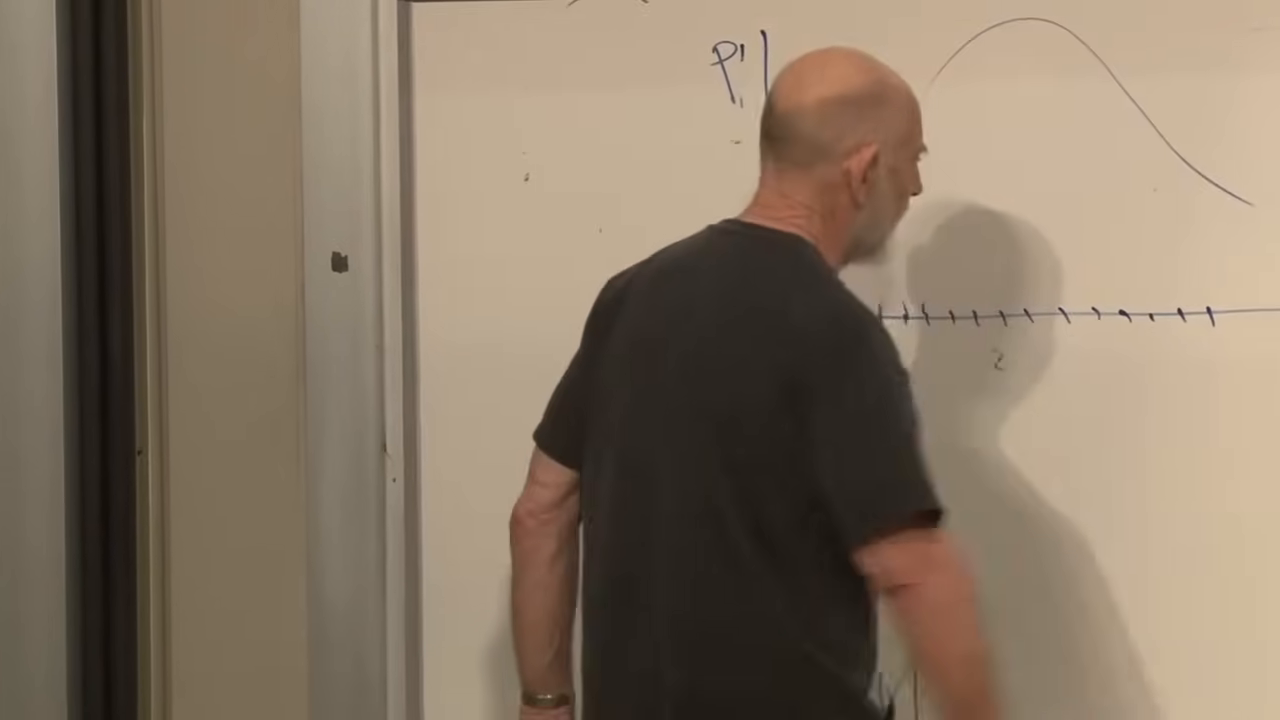
\includegraphics[width=0.92\textwidth]{lecture_01_figure_05.png}
\caption{Распределение вероятности по дискретным меткам состояний. Для энтропии важен разброс, а не точная форма кривой.}
\lectureframe{01:14:40}
\end{figure}

\begin{figure}[htbp]
\centering
\resizebox{\linewidth}{!}{%
\begin{tikzpicture}[>=Latex,scale=0.93]
\draw[->] (-4.2,0) -- (4.4,0) node[right] {state label \(i\)};
\draw[->] (-4,0) -- (-4,3.2) node[above] {$p_i$};
\foreach \x in {-3.6,-3.1,...,3.6}
  \draw (\x,0.08) -- (\x,-0.08);
\draw[very thick]
  plot[smooth] coordinates {
  (-3.7,0.12) (-3.0,0.28) (-2.3,0.72) (-1.6,1.45)
  (-0.9,2.25) (-0.2,2.65) (0.5,2.28) (1.2,1.55)
  (1.9,0.88) (2.7,0.38) (3.5,0.14)};
\draw (-1.8,-0.18) -- (-1.8,-0.5);
\draw (1.8,-0.18) -- (1.8,-0.5);
\draw[<->] (-1.8,-0.46) -- (1.8,-0.46);
\node at (0,-0.82) {effective spread};
\end{tikzpicture}
}
\caption{Узкое распределение несёт меньшую неопределённость, чем широкое. Энтропия должна характеризовать распределение в целом.}
\label{fig:sm1-probability-spread}
\end{figure}

Общее определение имеет вид
\begin{equation}
 S=-\sum_i p_i\log p_i.
 \label{eq:sm1-shannon-entropy}
\end{equation}
Используя \eqref{eq:sm1-expectation}, получаем
\begin{equation}
 S=-\langle\log p\rangle.
\end{equation}
Знак минус компенсирует тот факт, что \(\log p_i<0\), когда \(0<p_i<1\).

\subsection{Восстановление результата для равномерного случая}

Нужно проверить, что общая формула воспроизводит первое определение. Для незанятого состояния \(p_i=0\), тогда как \(\log p_i\) расходится. Однако произведение имеет хорошо определённое предельное значение
\begin{equation}
 \lim_{p\to0^+}p\log p=0.
 \label{eq:sm1-plogp-limit}
\end{equation}
Следовательно, состояния с нулевой вероятностью не вносят никакого вклада.

\begin{classroomqa}
\audiencequestion{Если \(p_i=0\), неужели этот член действительно обращается в нуль? Логарифм нуля равен минус бесконечности.}
\lecturerresponse{Этот член определяется пределом
\(\lim_{p\to0^+}p\log p\), который равен нулю. Множитель \(p\) стремится к нулю быстрее, чем логарифм расходится. Поэтому сколь угодно маловероятные состояния дают сколь угодно малые вклады, а точно невозможное состояние не даёт никакого вклада.
\lecturetimestamp{01:18:27--01:19:46}}
\end{classroomqa}

Для каждого из \(M\) занятых состояний \(p_i=1/M\). Следовательно,
\begin{align}
 S
 &=-\sum_{\mathrm{occupied}\ i}
 \frac1M\log\!\left(\frac1M\right)\\
 &=-M\frac1M\log\!\left(\frac1M\right)\\
 &=-\log\!\left(\frac1M\right)
 =\log M.
 \label{eq:sm1-entropy-check}
\end{align}
Общее выражение в точности совпадает со специальным. Более широкое распределение придаёт заметный вес большему числу альтернатив и потому имеет большую энтропию; более узкое распределение имеет меньшую энтропию.

\begin{figure}[htbp]
\centering
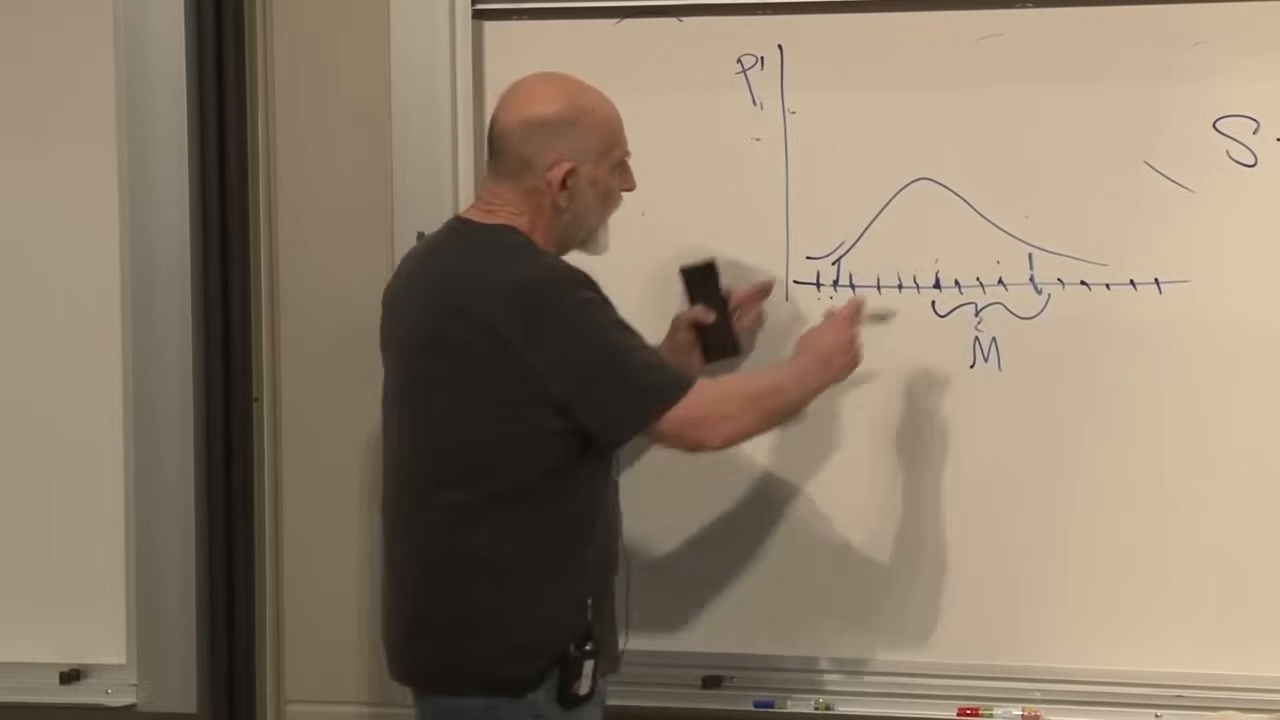
\includegraphics[width=0.92\textwidth]{lecture_01_figure_06.png}
\caption{Отмеченная ширина \(M\) подчёркивает связь между разбросом значимых вероятностей и энтропией.}
\lectureframe{01:16:42}
\end{figure}

Энтропия относится к распределению вероятности на пространстве состояний. Это не самостоятельная наблюдаемая величина, такая как энергия или импульс одного микросостояния. Точное состояние можно представить распределением, сосредоточенным на этом состоянии; тогда энтропия равна нулю, но при изменении состояния знания она меняется.

\section{Монеты, биты и явный подсчёт}

Пусть \(n\) — число монет. Число микроскопических конфигураций равно
\begin{equation}
 N=2^n.
 \label{eq:sm1-coin-state-count}
\end{equation}
Если о монетах ничего не известно, все \(2^n\) конфигурации равновероятны, и
\begin{equation}
 S_{\max}=\log(2^n)=n\log2.
 \label{eq:sm1-coin-max-entropy}
\end{equation}
Энтропия аддитивна по числу независимых монет.

При логарифмах по основанию \(2\) система с двумя состояниями, о которой ничего не известно, имеет энтропию в один бит. При натуральных логарифмах её энтропия равна \(\log2\). Единица измерения условна; лежащие в основе порядок и аддитивность не меняются.

В противоположном предельном случае, если состояние каждой монеты известно, ровно одна конфигурация имеет вероятность единица:
\begin{equation}
 S=0.
\end{equation}
Чем больше известно, тем меньше энтропия.

Теперь предположим, что ровно одна из \(n\) монет показывает решку, а все остальные — орла, причём положение решки неизвестно. Имеется \(n\) равновероятных конфигураций, по одной для каждого возможного положения решки, так что
\begin{equation}
 S=\log n.
 \label{eq:sm1-one-tail-entropy}
\end{equation}
Вообще говоря, это не целое кратное \(\log2\). Бит — удобная единица, а не утверждение, что любая энтропия бывает только целым числом бит.

\begin{classroomqa}
\audiencequestion{Появляется ли \(\log2\) только потому, что у каждой монеты есть два возможных состояния? Дал бы элемент с тремя состояниями \(\log3\)?}
\lecturerresponse{Именно. Элемент с \(k\) возможными состояниями, о котором известно лишь то, что все они равновероятны, даёт вклад \(\log k\). Двоичные переключатели особенно удобны в компьютерах, потому что физические переключатели естественным образом реализуют два устойчивых состояния и потому что 2 — наименьшее нетривиальное целое число.
\lecturetimestamp{01:29:55--01:30:48}}
\end{classroomqa}

\begin{classroomqa}
\audiencequestion{Какое основание логарифма здесь имеется в виду?}
\lecturerresponse{В этих физических формулах \(\log\) означает натуральный логарифм. Специалисты по теории информации часто используют основание \(2\), так что энтропия измеряется непосредственно в битах. Смена основания умножает любую энтропию на один и тот же постоянный коэффициент пересчёта и не меняет ни одного физического вывода.
\lecturetimestamp{01:30:49--01:32:06}}
\end{classroomqa}

\section{Энтропия в непрерывном фазовом пространстве}

Вернёмся к классическому фазовому пространству \(\Gamma\). Если плотность вероятности равномерна в области объёма \(V_\Gamma\) и вне её равна нулю, то аналог подсчёта \(M\) равновероятных состояний имеет вид
\begin{equation}
 S=\log\!\left(\frac{V_\Gamma}{V_0}\right).
 \label{eq:sm1-continuous-uniform}
\end{equation}
Здесь \(V_\Gamma\) — это объём в полном многомерном пространстве координат и импульсов, а не обычный пространственный объём. Фиксированный объём \(V_0\) — это эталонная ячейка фазового пространства, делающая логарифм безразмерным. При \(V_0=1\) получаем сокращённую запись \(S=\log V_\Gamma\), использовавшуюся на доске.

Для общей плотности вероятности \(P(q,p)\) дискретная сумма переходит в интеграл по фазовому пространству. Нормировка имеет вид
\begin{equation}
 \int_\Gamma d\Gamma\,P(q,p)=1,
 \label{eq:sm1-continuous-normalization}
\end{equation}
а энтропия равна
\begin{equation}
 S=-\int_\Gamma d\Gamma\,
 P(q,p)\log\!\bigl[P(q,p)V_0\bigr].
 \label{eq:sm1-continuous-entropy}
\end{equation}
Плотность — это вероятность, приходящаяся на ячейку фазового пространства. Концептуально \eqref{eq:sm1-continuous-entropy} по-прежнему измеряет, насколько широко распределена вероятность; для равномерной области она сводится к логарифму занятого объёма, измеренного в единицах эталонной ячейки. Замена этой фиксированной ячейки сдвигает любую непрерывную энтропию на одну и ту же аддитивную постоянную и оставляет разности энтропий неизменными.

\begin{classroomqa}
\audiencequestion{Почему обозначение координаты изменилось с \(x\) на \(q\)?}
\lecturerresponse{Никакого физического изменения нет. В классической механике для координат обычно используют либо \(x\), либо \(q\), а для сопряжённых импульсов — \(p\). Смена обозначения была лишь оговоркой; построение фазового пространства остаётся тем же.
\lecturetimestamp{01:37:10--01:37:39}}
\end{classroomqa}

Температура и распределение Больцмана намеренно отложены. Следующей задачей будет определить тепловое равновесие, а затем установить соответствующее ему распределение вероятностей.

\section{Вопросы о корреляции, аддитивности и информации}

\subsection{Корреляция означает, что одно измерение меняет распределение вероятностей для другой величины}

Полное незнание о независимых монетах приписывает каждой конфигурации равную вероятность. Измерение одной монеты тогда ничего не сообщает ни о какой другой монете. Их распределения остаются неизменными.

Ансамбль с одной решкой устроен иначе. Если у измеренной монеты выпала решка, то у всех остальных наверняка орёл. Если у измеренной монеты выпал орёл, то единственная решка должна находиться среди оставшихся \(n-1\) монет, так что каждая из оставшихся позиций имеет условную вероятность
\begin{equation}
\begin{aligned}
 p(&\text{tail at a specified remaining position}\\
   &\mid\text{measured head})=\frac{1}{n-1}.
\end{aligned}
 \label{eq:sm1-conditional-tail}
\end{equation}
Это и есть корреляция: узнав одну переменную, мы меняем распределение вероятностей, приписываемое другой.

\begin{classroomqa}
\audiencequestion{Предполагалась ли независимость монет в примерах с энтропией?}
\lecturerresponse{Только тогда, когда полное незнание представлялось равными вероятностями для всех \(2^n\) конфигураций. В этом случае измерение одной монеты не меняет распределений остальных. Пример с одной решкой явно коррелирован: измерение уточняет, что возможно в других местах. Указанная информация определяет, какое распределение вероятностей используется.
\lecturetimestamp{01:38:43--01:41:58}}
\end{classroomqa}

Пример с несвязанными циклами имеет ту же логическую форму. Измерение сохраняющейся метки \(+1\) или \(-1\) ограничивает все последующие состояния одним сектором. Условление по сохраняющейся информации изменяет допустимое распределение.

Энтропия аддитивна для некоррелированных систем. Если
\begin{equation}
 p_{ij}=p_i^{(A)}p_j^{(B)},
\end{equation}
то
\begin{align}
 S_{AB}
 &=-\sum_{i,j}p_i^{(A)}p_j^{(B)}
 \log\!\left[p_i^{(A)}p_j^{(B)}\right]\\
 &=S_A+S_B.
 \label{eq:sm1-entropy-additivity}
\end{align}
Корреляции препятствуют такой факторизации и уменьшают независимую неопределённость пары.

В качестве упражнения представьте себе ряд двоичных переменных, для которых верхнее состояние означает, что каждый сосед с вероятностью три четверти находится в нижнем состоянии. Измерение в одном узле немедленно изменяет то, что известно о ближайших узлах. Такое распределение коррелировано, и его энтропию нельзя найти, просто складывая изолированные одноузловые энтропии без учёта этих корреляций.

\subsection{Больцман, Шеннон и квантовая неопределённость}

\begin{classroomqa}
\audiencequestion{Как более ранняя термодинамическая энтропия связана с информационно-теоретической энтропией Шеннона?}
\lecturerresponse{В обоих случаях появляется одна и та же функциональная форма:
\(-\sum_i p_i\log p_i\). Шеннон обычно использовал основание \(2\), тогда как физики обычно используют натуральные логарифмы и восстанавливают постоянную Больцмана, когда энтропия выражается в термодинамических единицах. Математическое различие сводится лишь к постоянному коэффициенту пересчёта, хотя физические вопросы, задающие вероятности, могут быть очень разными.
\lecturetimestamp{01:44:05--01:46:06}}
\end{classroomqa}

Для равновероятных микросостояний термодинамическую формулу часто записывают в виде
\begin{equation}
 S_{\mathrm{thermo}}=k_{\mathrm B}\log W,
 \label{eq:sm1-boltzmann-formula}
\end{equation}
где \(W\) — число доступных микросостояний. В единицах, где \(k_{\mathrm B}=1\), это в точности \(S=\log W\). Постоянная Больцмана служит коэффициентом пересчёта между единицами температуры и единицами энергии; естественный микроскопический масштаб температуры — энергия.

\begin{classroomqa}
\audiencequestion{Является ли эта энтропия просто иной формой принципа неопределённости Гейзенберга?}
\lecturerresponse{Нет. Рассматриваемая здесь энтропия измеряет неопределённость в распределении вероятностей по возможным состояниям. На языке квантовой механики это неопределённость смешанного состояния, а не внутренняя неопределённость измерения, которая может сохраняться даже для чистого состояния. Эти два понятия необходимо различать.
\lecturetimestamp{01:46:07--01:47:31}}
\end{classroomqa}

\section{Что было установлено}

Исходным пунктом была не случайность в самих законах. Детерминистическая динамика в сочетании с неполным знанием начального состояния уже порождает вероятности. Одна орбита задаёт веса через время пребывания в каждом состоянии; несвязанные орбиты выявляют сохраняющиеся величины и требуют априорных весов между секторами. Допустимые микроскопические законы сохраняют различимость состояний; в конечном пространстве состояний это означает по одной входящей и по одной исходящей стрелке в каждом состоянии, а в непрерывной механике выражается теоремой Лиувилля.

Эта структура приводит сначала к
\begin{equation}
 S=\log M
\end{equation}
для \(M\) занятых равновероятных состояний, затем к
\begin{equation}
 S=-\sum_i p_i\log p_i,
\end{equation}
и наконец к его интегралу по фазовому пространству. Энтропия фиксирует распределение вероятностей и, следовательно, состояние знания. Детальная информация сохраняется микроскопическим законом даже тогда, когда практическое огрублённое описание теряет её из виду.

Сохранение энергии даёт первый закон, тогда как аддитивность энергий подсистем требует пренебрежимо малой энергии взаимодействия. Энтропия аддитивна при аналогичном условии: распределения вероятностей подсистем должны быть некоррелированными. Эти два вида аддитивности подготавливают следующий шаг, на котором тепловое равновесие, температура и распределение Больцмана свяжут энергию с вероятностью.